%!TEX program = xelatex

\documentclass[11pt,titlepage]{report}
%!TEX root = main.tex

\usepackage[T1]{fontenc}
\usepackage{lmodern}
\usepackage[svgnames]{xcolor}
\usepackage{fontspec} % XeLaTeX required!
\usepackage{graphicx}
\usepackage{circuitikz}
\usepackage{tikz}
\usepackage{pifont}
\usepackage[some]{background}
\usepackage{xltxtra} 
\usepackage{setspace}
\usepackage[absolute]{textpos}
\usepackage[latin1]{inputenc}
\usepackage[english]{babel}
\usepackage{graphicx}
\usepackage{wrapfig}
\usepackage{fullpage}
\usepackage[margin=1in]{geometry}
\usepackage{float}
\usepackage{url}
\usepackage{multicol}
\usepackage{hyperref}
\usepackage{titlepic}
\usepackage{standalone}
\usepackage{siunitx}
\usepackage{booktabs}
\usepackage{amsmath}
\usepackage{unicode-math}
\usepackage{verbatim}
\usepackage{enumitem}
\usepackage{listings}
\usepackage{multirow}
\usepackage{pgfplots}
\pgfplotsset{compat=1.8}
\usepackage{caption} 
\usepackage[parfill]{parskip}
\usepackage{import}
\usepackage[backend=bibtexu,texencoding=utf8,bibencoding=utf8,style=ieee,sortlocale=en_GB,language=auto]{biblatex}
\usepackage[strict,autostyle]{csquotes}
\usepackage[final]{pdfpages}
\usepackage{subcaption}
\usepackage{ifplatform}
%\captionsetup[table]{skip=10pt}


% Fix for includepdf bug in Mac OS X
\newcommand{\insertpdfpath}[1]{
	\ifwindows
	\newcommand{\insertpdf}[2]{\includepdf[pages=##1]{##2}}
	\else
	\newcommand{\insertpdf}[2]{\includepdf[pages=##1]{#1/##2}}
	\fi
}

%set fonts
\setmainfont[Ligatures=TeX]{Myriad Pro}
\setmathfont{Asana Math}
\setmonofont{Lucida Console}

\usepackage{titlesec, color}
\renewcommand{\familydefault}{\sfdefault} %set font family
\renewcommand{\arraystretch}{1.2} %set table vertical spacing
\setlength\parindent{0pt} %no paragraph indent
\hypersetup{ %setup hyperlinks
    colorlinks,
    citecolor=black,
    filecolor=black,
    linkcolor=black,
    urlcolor=black
}

%redesign chapter headings
\definecolor{gray75}{gray}{0.75}
\newcommand{\chapternumber}{\thechapter}
\newcommand{\hsp}{\hspace{20pt}}
\titleformat{\chapter}[hang]{\Huge\bfseries}{\chapternumber\hsp\textcolor{gray75}{|}\hsp}{0pt}{\Huge\bfseries}

%Redefine appendix headers
\renewcommand{\appendixname}{Appendix}
\renewcommand{\appendixtocname}{Appendices}
\renewcommand{\appendixpagename}{Appendices}

%For code listings
\definecolor{black}{rgb}{0,0,0}
\definecolor{browntags}{rgb}{0.65,0.1,0.1}
\definecolor{bluestrings}{rgb}{0,0,1}
\definecolor{graycomments}{rgb}{0.4,0.4,0.4}
\definecolor{redkeywords}{rgb}{1,0,0}
\definecolor{bluekeywords}{rgb}{0.13,0.13,0.8}
\definecolor{greencomments}{rgb}{0,0.5,0}
\definecolor{redstrings}{rgb}{0.9,0,0}
\definecolor{purpleidentifiers}{rgb}{0.01,0,0.01}


\lstdefinestyle{csharp}{
language=[Sharp]C,
showspaces=false,
showtabs=false,
breaklines=true,
showstringspaces=false,
breakatwhitespace=true,
escapeinside={(*@}{@*)},
columns=fullflexible,
commentstyle=\color{greencomments},
keywordstyle=\color{bluekeywords}\bfseries,
stringstyle=\color{redstrings},
identifierstyle=\color{purpleidentifiers},
basicstyle=\ttfamily\small}

\lstdefinestyle{c}{
language=C,
showspaces=false,
showtabs=false,
breaklines=true,
showstringspaces=false,
breakatwhitespace=true,
escapeinside={(*@}{@*)},
columns=fullflexible,
commentstyle=\color{greencomments},
keywordstyle=\color{bluekeywords}\bfseries,
stringstyle=\color{redstrings},
identifierstyle=\color{purpleidentifiers},
}

\lstdefinestyle{matlab}{
language=Matlab,
showspaces=false,
showtabs=false,
breaklines=true,
showstringspaces=false,
breakatwhitespace=true,
escapeinside={(*@}{@*)},
columns=fullflexible,
commentstyle=\color{greencomments},
keywordstyle=\color{bluekeywords}\bfseries,
stringstyle=\color{redstrings},
identifierstyle=\color{purpleidentifiers}
}

\lstdefinestyle{vhdl}{
language=VHDL,
showspaces=false,
showtabs=false,
breaklines=true,
showstringspaces=false,
breakatwhitespace=true,
escapeinside={(*@}{@*)},
columns=fullflexible,
commentstyle=\color{greencomments},
keywordstyle=\color{bluekeywords}\bfseries,
stringstyle=\color{redstrings},
identifierstyle=\color{purpleidentifiers}
}

\lstdefinestyle{xaml}{
language=XML,
showspaces=false,
showtabs=false,
breaklines=true,
showstringspaces=false,
breakatwhitespace=true,
escapeinside={(*@}{@*)},
columns=fullflexible,
commentstyle=\color{greencomments},
keywordstyle=\color{redkeywords},
stringstyle=\color{bluestrings},
tagstyle=\color{browntags},
morestring=[b]",
  morecomment=[s]{<?}{?>},
  morekeywords={xmlns,version,typex:AsyncRecords,x:Arguments,x:Boolean,x:Byte,x:Char,x:Class,x:ClassAttributes,x:ClassModifier,x:Code,x:ConnectionId,x:Decimal,x:Double,x:FactoryMethod,x:FieldModifier,x:Int16,x:Int32,x:Int64,x:Key,x:Members,x:Name,x:Object,x:Property,x:Shared,x:Single,x:String,x:Subclass,x:SynchronousMode,x:TimeSpan,x:TypeArguments,x:Uid,x:Uri,x:XData,Grid.Column,Grid.ColumnSpan,Click,ClipToBounds,Content,DropDownOpened,FontSize,Foreground,Header,Height,HorizontalAlignment,HorizontalContentAlignment,IsCancel,IsDefault,IsEnabled,IsSelected,Margin,MinHeight,MinWidth,Padding,SnapsToDevicePixels,Target,TextWrapping,Title,VerticalAlignment,VerticalContentAlignment,Width,WindowStartupLocation,Binding,Mode,OneWay,xmlns:x}
}

\lstdefinestyle{matlab}{
language=Matlab,
showspaces=false,
showtabs=false,
breaklines=true,
showstringspaces=false,
breakatwhitespace=true,
escapeinside={(*@}{@*)},
columns=fullflexible,
commentstyle=\color{greencomments},
keywordstyle=\color{bluekeywords}\bfseries,
stringstyle=\color{purpleidentifiers},
identifierstyle=\color{purpleidentifiers}
}

%defaults
\lstset{
basicstyle=\ttfamily\small,
extendedchars=false,
numbers=left,
numberstyle=\ttfamily\tiny,
stepnumber=1,
tabsize=4,
numbersep=5pt
}
\addbibresource{../library/bibliography.bib}

\begin{document}
\begin{appendices}
\renewcommand{\chapternumber}{\appendixname\space\thechapter}

% Content:
% - Signal filtering
% - Using the Doppler effect to increase measurement accuracy
% - Introduction to numerically solving differential equations
\chapter{Charging system}
\label{app:chargingsystem}

\subsection{Diodes}
For the diodes we again calculate the total power loss. When assuming that the output voltage is near constant, the static dissipation, in context of the inverter, is given by
\begin{equation}
\label{eq:ass1-diode-static-power}
	P_s = I V_{fw} D_{d}
\end{equation}
in which $I$ represents the current flowing through the diodes, $V_{fw}$ the forward voltage drop and $D_{d}$ the \textit{diode duty cycle}. The diode duty cycle determines the percentage of time in which current flows through the diode with respect to the switching frequency. $D_{d}$ is given by
\begin{equation}
\label{eq:ass1-diode-dutycycle}
	D_d = \frac{1}{2}+\arcsin{ \left( \frac{V_{min}}{V_{max}}-1 \right) }
\end{equation}
in which the minumum and maximum output voltage of the inverter is represented by $V_{min}$ and $V_{max}$. The dynamic power dissipation is per diode given by
\begin{equation}
\label{eq:ass1-diode-dynamic-power}
	P_s = C_j V_{DS}^2
\end{equation}
in which the junction capacitance is represented by $C_j$. The combination of these formulas yields the total power dissipation.

\chapter{Inverter Schematics}
\label{app:schematics}
The following pages will contain the final design of the inverter.
\insertpdf{1-6}{resources/schematics-rc.pdf}

\subsection{PCB Layout}
\label{app:pcb_layout}
The following pages will contain a two dimensional view of each layer of the PCB. Also, a combined view is included.
\insertpdf{1-3}{resources/pcb-layout-rc.pdf}

\subsection{Inverter Waveforms}
Figure~\ref{fig:app-osc-coil-primary} and Figure~\ref{fig:app-osc-coil-secondary} show the results of the measurements of the inverter.
\label{app:waveforms}
\begin{figure}[H]
	\begin{center}
		\begin{subfigure}[h]{0.48\textwidth}
			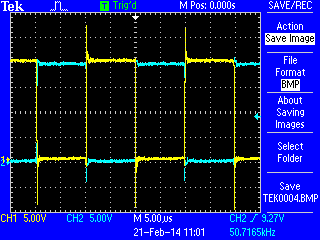
\includegraphics[width=\textwidth]{resources/osc-coil-primary.png}
			\caption{Voltage of the two ends of the primary coil with respect to ground}
			\label{fig:app-osc-coil-primary}
		\end{subfigure}
		\quad
		\begin{subfigure}[h]{0.48\textwidth}
			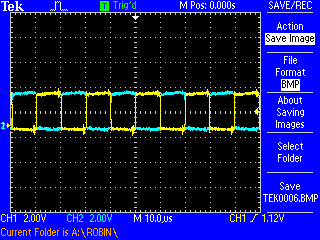
\includegraphics[width=\textwidth]{resources/osc-coil-secondary.png}
			\caption{Voltage of the two ends of the secondary coil with respect to ground}
			\label{fig:app-osc-coil-secondary}
		\end{subfigure}
	\end{center}
	\caption{Inverter voltage waveforms at primary and secondary side}
\end{figure}




\chapter{Signal filtering}
\label{app:signal-filtering}
\section{Prediction filter}
To process measured values, consistent sensor output is required. However, every now and then, the sensors output unrealistic values. To overcome this problem, we have created a finite impulse response filter which would predict the next measured value. If the measured value differs too much from the predicted value, the measured value is replaced.

Let the measured distances be $x_i$ with $i \in [0,n]$. If the sample time is $T$, then the current observed speed is given by

\begin{equation}
	v_n = \frac{x_{n} - x_{n-1}}{T}.
\end{equation}

The current observed acceleration is given by

\begin{equation}
	a_n = \frac{v_n - v_{n-1}}{T} = \frac{x_{n} - 2 x_{n-1} + x_{n-2}}{T^2}.
\end{equation}

Assuming constant speed and acceleration, the predicted next distance is given by

\begin{equation}
	y_{n+1} = x_{n} + v_n T + \frac{1}{2} a T^2 = \frac{5}{2} x_n - 2 x_{n-1} + \frac{1}{2} x_{n-2}= x_n \ast h_n
\end{equation}

in which

\begin{equation}
	h_n = \left\{
	\begin{array}{l l}
		\frac{5}{2} & \quad n = 0, \\
		-2 & \quad n = 1, \\
		\frac{1}{2} & \quad n = 2, \\
		0 & \quad \text{elsewhere}.
	\end{array}
	\right.
\end{equation}

Note that

\begin{equation}
	E[y_n] = \left( \sum_{n=-\infty}^{\infty} h_n \right) E[x_n] = E[x_n].
\end{equation}

\section{Noise filtering}

Consider a ordinary second-order low pass filter with transfer function

\begin{equation}
	\frac{Y(s)}{X(s)}=\frac{1}{(1+(2 \pi f_{fall})^{-1} s)^2}.
\end{equation}

Defining

\begin{equation}
	\alpha = (2 \pi f_{fall} T_s)^{-1}
\end{equation}

and rewriting the transfer function yields

\begin{equation}
	Y(s) \left(\frac{\alpha^2}{T_s^2} s^2 + 2 \frac{\alpha}{T_s} s + 1 \right) = X(s).
\end{equation}

Inverse Laplace transforming and converting to discrete time using

\begin{equation}
	\frac{d}{dt}f(t) = \frac{f_n - f_{n-1}}{T_s}
\end{equation}

yields us a second-order discrete time infinite impulse response low pass filter given by

\begin{equation}
	y_{n+1} = c_1 y_n + c_2 y_{n-1} + c_3 x_{n+1}
\end{equation}

in which

\begin{align}
	c_1 &= \frac{2 \alpha^2 + 2 \alpha}{\alpha^2 + 2 \alpha + 1}, \\
	c_2 &= \frac{-\alpha^2}{\alpha^2 + 2 \alpha + 1}, \\
	c_3 &= \frac{1}{\alpha^2+2 \alpha + 1}.
\end{align}

Note that

\begin{equation}
	c_1 + c_2 + c_3 = 1.
\end{equation}

It is important to realize that applying such a filter introduces delay. The delay $T(f)$ could be estimated by calculating the phase shift $\phi(f)$ of the transfer function and using

\begin{equation}
	T(f) = \frac{-1}{2 \pi f} \phi(f).
\end{equation}

\chapter{Using the Doppler effect to increase measurement accuracy}
\label{app:doppler}
Let us consider KITT driving with velocity $v'$ at a non-moving object at distance $x$. One can use the classical Doppler effect to accurately determine the distance to this non-moving object. The wavelength $\lambda'$ of the wave, which will be sent out by KITT's ultrasonic sensor, is given by

\begin{equation}
	\lambda' = \lambda - \Delta \lambda = T (v - v'),
\end{equation}

in which the speed of sound is given by $v$ and the period at which the waves are sent out by $T$. The sent-out waves will reflect at the non-moving object and will consequently be sensed by KITT's sensors. Their wavelength will then be given by

\begin{equation}
	\lambda'' = \lambda' - \Delta \lambda = T (v - 2 v').
\end{equation}

The period $T'$ of the incoming waves is thus

\begin{equation}
	T' = \frac{\lambda''}{v} = T \frac{v - 2 v'}{v}.
\end{equation}

One can use the ratio of the periods of transmitted and received waves to determines the vehicle's speed.

\begin{equation} \label{eq:ass-2-vel-car}
 	v' = \left(1-\frac{T'}{T} \right) \frac{v}{2}
 \end{equation}

Between the transmission and reception of the waves, a time $T_s$ will have elapsed and the vehicle will have moved a distance $v' T_s$. Thus, the total distance a wave will have travelled is given by

\begin{equation}
	x_{wave} = 2 d - T_s v' = T_s v.
\end{equation}

Solving for $x$ yields

\begin{equation} \label{eq:ass-2-pre-dist-car}
	x = \frac{v T_s}{4} \left(3 - \frac{T'}{T} \right).
\end{equation}

If the processing time of the recieved signals is given by $T_p$, then, after processing, the distance of the car to the wall is calculated by

\begin{equation}
	x_{car} = d-(T_s +T_p) v'.
\end{equation}

Substituting Equations \ref{eq:ass-2-vel-car} and \ref{eq:ass-2-pre-dist-car} yields an expression for the actual distance of the car to the non-moving object. This expression is given by

\begin{equation}
	x_{car} = \frac{v}{4 T} \left((T'+T) T_s + 2 T_p (T'-T)  \right).
\end{equation}

The linearized relative uncertainty, given by

\begin{equation}
	u_{d,rel} = \frac{1}{x_{car}} \left( \frac{d x_{car}}{d T} \Delta T + \frac{d x_{car}}{d T'} \Delta T' + \frac{d x_{car}}{d T_p} \Delta T_p + \frac{d x_{car}}{d T_s} \Delta T_s \right),
\end{equation}

yields

\begin{equation}
	u_{d,rel} = \frac{
		-T(T_s + 2 T_p) u_T + T^2 (u_{T_s} - 2 u_{T_p}) + T \left( (T_s + 2 T_p) u_{T'} + T' (u_{T_s} + 2 u_{T_p}) \right)
	}{
		T \left( (T'+T)T_s + 2 T_p (T'-T) \right)
	}.
\end{equation}

If one can assume that

\begin{equation}
	\frac{u_T}{T} = \frac{u_{T'}}{T'} = \frac{u_{T_p}}{T_p} = \frac{u_{T_s}}{T_s}=r,
\end{equation}

then the linearized relative uncertainty $u_{d,rel}$ magically simplifies to $r$. An attentive reader would be able to verify this result by inspection. \textit{Mathematica 9 Student Edition} was used for aid in algebraic manipulation and simplification of the equations. Unfortunately, the signal processing of the ultrasonic sensors is handled by KITT.

\chapter{Numerically solving KITT}

\textit{Note that this section does not give mathematically formal derivations and statements. This section is meant to tickle the readers intuition.}

The solution of our state-space model is obtained by solving

\begin{equation}
	\dot{\vec{x}}=\mat{A}\vec{x}+\mat{B}\vec{u}.
\end{equation}

We can simplify this problem to 

\begin{equation}
	\dot{x}=f(x).
\end{equation}

We can rewrite this equation using Taylor series expansion.

\begin{align}
	\frac{dx}{dt} &= f(x), \\
	x(t_0+\Delta t) &\approx
		x(t_0)+
		\left. \Delta t \frac{dx}{dt} \right|_{t=t_0}+
		\frac{\Delta t^2}{2}\left. \frac{d^2x}{dt^2} \right|_{t=t_0}+
		\text{h.o.t.}, \\
	x(t_0+\Delta t) &\approx
		x(t_0)+
		\Delta t \left(
			\left. \frac{dx}{dt} \right|_{t=t_0}+
			\frac{\Delta t}{2}\left. \frac{d^2x}{dt^2} \right|_{t=t_0}
		\right) + \text{h.o.t.} \label{eq:app-approx}
\end{align}

Evaluating the derivative at $t=t_0+\Delta t$ yields

\begin{equation}
	\left. \frac{dx}{dt} \right|_{t=t_0+\Delta t} = 
		\left. \frac{dx}{dt} \right|_{t=t_0} +
		\Delta t \left. \frac{d^2x}{dt^2} \right|_{t=t_0} +
		\text{h.o.t.}
\end{equation}

One might notice that the first two terms of Equation~\ref{eq:app-approx} can be written as a linear combination

\begin{equation}
	a \left. \frac{dx}{dt} \right|_{t=t_0} +
	b \left. \frac{dx}{dt} \right|_{t=t_0+\Delta t} =
		\left. \frac{dx}{dt} \right|_{t=t_0}+
		\frac{\Delta t}{2}\left. \frac{d^2x}{dt^2} \right|_{t=t_0},
\end{equation}

\begin{equation}
	\begin{bmatrix}
		1 & 1 \\
		0 & 1 
	\end{bmatrix} \begin{bmatrix}
		a \\
		b 
	\end{bmatrix} = \begin{bmatrix}
		1 \\
		1/2
	\end{bmatrix} \Leftrightarrow \begin{bmatrix}
		a \\
		b
	\end{bmatrix} = \begin{bmatrix}
		1/2 \\ 
		1/2
	\end{bmatrix}.
\end{equation}

This indicates that the a second-order approximation is given by a linear combination of the slope at $t=t_0$ and $t=t_0+\Delta t$. This result yields us Heun's method, which is a second-order Runge-Kutta method. 

\chapter{Source code}
\inputfrom{../../}{sourcecode}

\end{appendices}
\end{document}